\documentclass[12pt]{amsart}
%\usepackage{tweaklist}
\usepackage{cancel}
\usepackage{xspace}
\usepackage[utf8]{inputenc}
\usepackage{graphicx}
\usepackage{multicol}
\usepackage{subfig}
\usepackage{amsmath}
\usepackage{amssymb}
\usepackage[a4paper,width=160mm,top=18mm,bottom=21mm,includeheadfoot]{geometry}
\usepackage{booktabs}
\usepackage{array}
\usepackage{verbatim}
\usepackage{caption}
% \usepackage{natbib}

\usepackage{float}
\usepackage{pdflscape}
\usepackage{mathtools}
\usepackage[usenames,dvipsnames]{xcolor}
\usepackage{afterpage}
\usepackage{tikz}
\usepackage[hyperfootnotes=false, bookmarks=true, unicode=true, pdftitle={Ethereum Yellow Paper: a formal specification of Ethereum, a programmable blockchain}, pdfauthor={Dr. Gavin Wood},pdfkeywords={Ethereum, Yellow Paper, blockchain, virtual machine, cryptography, decentralised, singleton, transaction, generalised},pdfborder={0 0 0.5 [1 3]}]{hyperref}
%,pagebackref=true

\usepackage{tabu} %requires array.
\def\els@aparagraph[#1]#2{\elsparagraph[#1]{#2}}
\def\els@bparagraph#1{\elsparagraph*{#1}}
\newcommand\eatpunct[1]{}
%This should be the last package before \input{Version.tex}
\PassOptionsToPackage{hyphens}{url}\usepackage{hyperref}
% "hyperref loads the url package internally. Use \PassOptionsToPackage{hyphens}{url}\usepackage{hyperref} to pass the option to the url package when it is loaded by hyperref. This avoids any package option clashes." Source: <https://tex.stackexchange.com/questions/3033/forcing-linebreaks-in-url/3034#comment44478_3034>.
% Note also this: "If the \PassOptionsToPackage{hyphens}{url} approach does not work, maybe it's "because you're trying to load the url package with a specific option, but it's being loaded by one of your packages before that with a different set of options. Try loading the url package earlier than the package that requires it. If it's loaded by the document class, try using \RequirePackage[hyphens]{url} before the document class." Source: <https://tex.stackexchange.com/questions/3033/forcing-linebreaks-in-url/3034#comment555944_3034>.
% For more information on using the hyperref package, refer to e.g. https://en.wikibooks.org/w/index.php?title=LaTeX/Hyperlinks&stable=0#Hyperlink_and_Hypertarget.

\makeatletter
 \newcommand{\linkdest}[1]{\Hy@raisedlink{\hypertarget{#1}{}}}
\makeatother
\usepackage{seqsplit}

% For formatting
%\usepackage{underscore}
%\usepackage{lipsum} % to generate filler text for testing of document rendering
\usepackage[english]{babel}
\usepackage[autostyle]{csquotes}
\MakeOuterQuote{"}

\usepackage[final]{microtype} % https://tex.stackexchange.com/questions/75140/is-it-possible-to-make-latex-mark-overfull-boxes-in-the-output#comment382776_75142
\usepackage{lastpage}
\usepackage{footnote}
\usepackage{caption}
\definecolor{Orange}{rgb}{0.241,0.349,0.090}
\usepackage{bbding}
\usepackage{shortvrb}
%% \usepackage{draftwatermark}
%% \SetWatermarkText{Esborrany}
%% \SetWatermarkScale{0.5}
%% \usepackage{tocloft}
% \usepackage{hyperref}
% \usepackage{bookmark}
\usepackage[titletoc]{appendix}


% \input{Version.tex}
% Default rendering options
\definecolor{pagecolor}{rgb}{1,0.98,0.9}
\def\YellowPaperVersionNumber{unknown revision}
\IfFileExists{Options.tex}{\input{Options.tex}}

\newcommand{\hcancel}[1]{%
    \tikz[baseline=(tocancel.base)]{
        \node[inner sep=0pt,outer sep=0pt] (tocancel) {#1};
        \draw[black] (tocancel.south west) -- (tocancel.north east);
    }%
}%


\DeclarePairedDelimiter{\ceil}{\lceil}{\rceil}
\newcommand*\eg{e.g.\@\xspace}
\newcommand*\Eg{e.g.\@\xspace}
\newcommand*\ie{i.e.\@\xspace}
%\renewcommand{\itemhook}{\setlength{\topsep}{0pt}  \setlength{\itemsep}{0pt}\setlength{\leftmargin}{15pt}}


\title{Wireless service accounting based on Ethereum state channels
- Master Thesis}

\author{
  A. Egio,
  L. González, A. Pardo, T. Romero
}


\begin{document}

\pagecolor{pagecolor}


\begin{abstract}
  \begin{center}
    This document contains authors' ``\textit{Blockchain
      technologies master}''\footnote{UPC School
      of Professional \& Executive Development}
    final thesis. The project described in the document
    consists on a technological proof
    of concept of an internet access service consumption
    using a state channel smart contract as
    mean of payment. After a brief
    introduction, there's a first motivation of
    the use case included;
    in the following sections
    there's a detailed explanation of
    the architecture, implementation and
    security considerations;
    after that it is described a more
    general approach on using blockchain technologies
    and state channels in particular to provide
    mechanisms to reduce advanced wireless
    (i. e. 5G) services market friction between neutral host
    providers, virtual operators and operators
    licensing spectrum bands to nations' governments;
    guarantee transparency to consumers,
    and provide a fully GDPR compliant
    schema using a self-sovereign identity system.
  \end{center}
\end{abstract}

\maketitle

\tableofcontents

\newpage

\setlength{\columnsep}{20pt}
\begin{multicols}{2}
\section{Introduction}\label{sec:introduction}

\vspace{0.35cm}
As exposed in \cite{spectrumnh} although radio spectrum
``\textit{is often
  referred to as a `scarce resource`}'' there are
spectrum management strategies
being researched to improve and
support a brand new model of services
into the market; in particular there are
multiple 5G\cite{5g} innovative projects and initiatives
that try to solve this using Software
Defined Network\cite{sdns}
and Network Function Virtualization\cite{nfv}.

\vspace{0.35cm}

Since spectrum is a scarce resource, it can
be tokenized being suited this
way for blockchain/DLT technologies business models;
in addition, since
atmospheric spectrum can be considered a public
asset, it's managed in last terms by nations' governments
and it's licensing and management should feature
a high level of transparency and at the same time
allow for efficiency and fair-competition making it
feasible to model on public blockchain systems.

\vspace{0.35cm}

Taking this into account, lead the authors' to develop
a first bottom-up proof of concept of a simple system
demonstrating how can a wireless WiFi hotspot
deployed on a commodity hardware asset\cite{RaspberryPi19}
be managed to allow users to access the internet
paying in exchange for Ethereum on a public network.

\vspace{0.35cm}

One of the first intiatives to create
a bandwidth reselling market was La Fonera\cite{fon}
back in 2006. Main goal of the initiative was
to allow ADSL users to share unused bandwidth using
a specific WiFi hotspot deployed on an ad-hoc
built router.

\begin{center}
  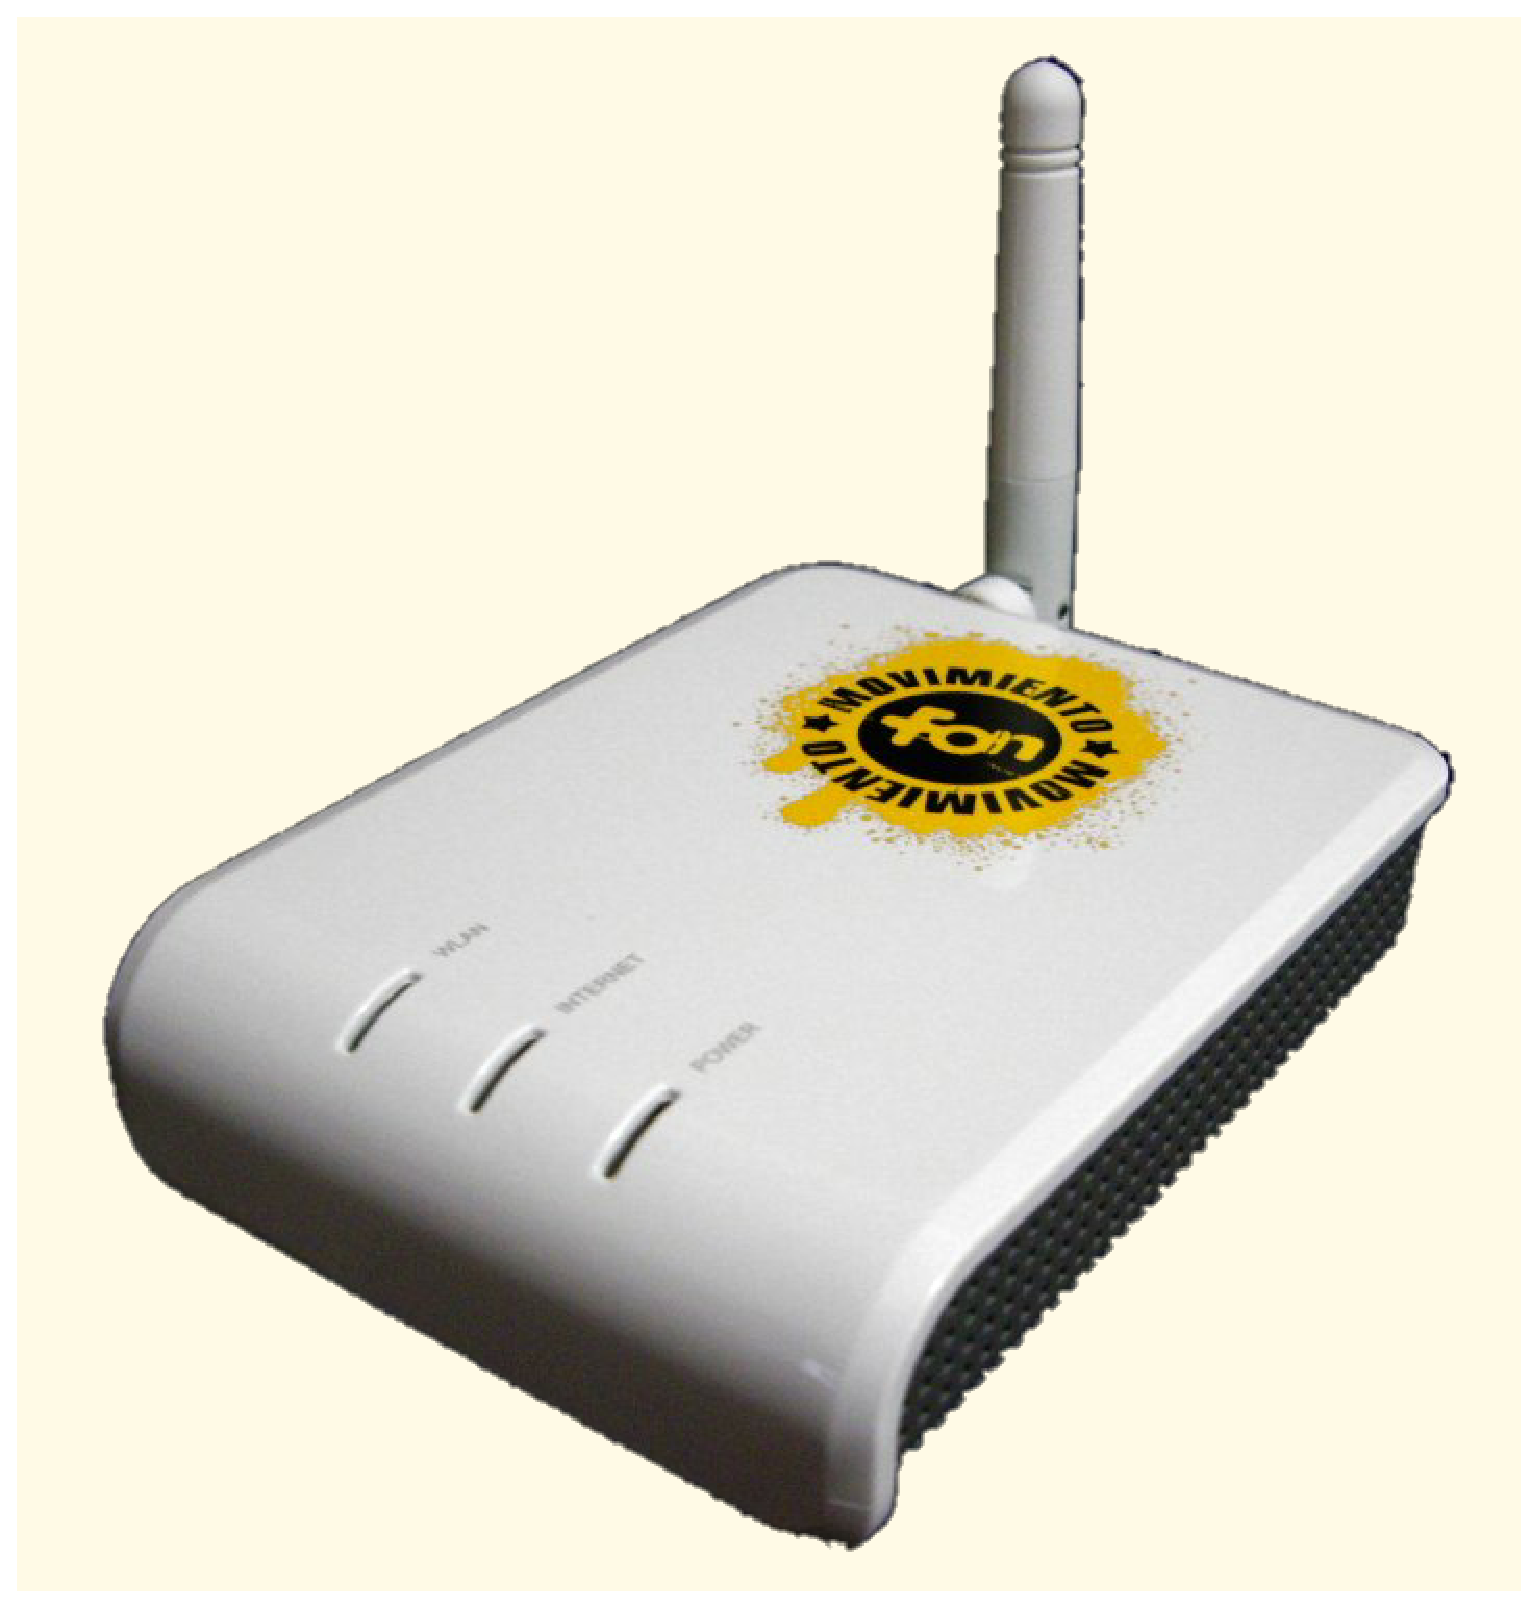
\includegraphics[keepaspectratio, width=0.2\textwidth]{images/lafonera-sourcewikipedia.eps}
  \\
  Figure 1. \textit{La Fonera's initial project router.}
\end{center}

\vspace{0.35cm}

A more recent project like Hotspot Me\cite{hotspotme}
and also very aligned with the technological demonstration
described in this document consist on using mobile
APIs to allow a users to share WiFi hotspot tethering
to users nearby in exchange for ETH supported by a
micro-payment channel contract.


\section{Technological background}\label{ch:bc}

\vspace{0.35cm}

Blockchain technologies support a ledger of records in
continuous growth called blocks.
They are linked and secured by
cryptography. Adopt the P2P protocol
(\textit{peer-to-peer}) in order to be distributed
with not a single point of failure.

\vspace{0.35cm}

The consensus mechanism ensures a common order
of unambiguous transactions and
blocks, and guarantees integrity and
blockchain consistency a
through geographically distributed nodes.
By its design, the blockchain has characteristics
such as: decentralization, integrity and auditability.
The blockchain can serve as a new
type of software connector, which should be considered
as a possible decentralized alternative to storage
of existing centralized shared data.

\vspace{0.35cm}

In addition, depending on the different levels of
access permission, block chains can
split into two types:
1) public (such as Bitcoin and Ethereum); Y
2) private (such as Hyperledger). Blockchain serves
as a platform for smart contracts
(hereinafter, \ textit {smart contracts}).
For example, programmed in the Solidity language of
Ethereum, stay and run.
Blockchain is a technology concept
DLT distributed ledger
(\ textit {distributed ledger technology}).
It can be integrated into multiple business areas.

%% \textit{ETH-Paid hotspot provider} (E-Php).
%% \\
%% \\
%% \textit{Hotspot handler} (hh).
%% \\
%% \\
%% \textit{Upstream Internet Service Provider} (U-ISP).
%% \\

\section{Technological Proof of Concept description}

\subsection{Architecture}
\label{ch:architecture}
\vspace{0.35cm}

In order to support the PoC a
Raspberry Pi 3 Model B (see figure 2) has been used
as a single board computer to provide a WiFi access point using
hostapd\cite{hostapd} daemon over Raspberry's WiFi chipset.
Raspberry Pi was also connected using ethernet cable
to an optical fiber commercial router.

\begin{center}
%\begin{figure}[h]
%  \centering
  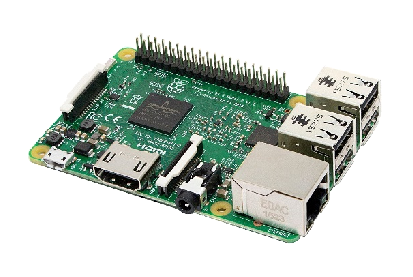
\includegraphics[keepaspectratio, width=0.2\textwidth]{images/rpi3modelb-sourceamazon.eps}
%  \caption{Figura 2. Raspberry Pi 3 Modelo B. Fuente: [Raspberry 18]}
%\end{figure}
\\
Figure 2. Raspberry Pi 3 Model B. Source: \cite{RaspberryPi3}
\\
\end{center}

\vspace{0.35cm}

Dnsmasq\cite{dnsmasq} was used
as dynamic host configuration server for the wireless
network and
iptables\cite{iptables} was used as a firewall running
both inside the Raspberry; by default, iptables
was configured to
drop all packet
forwarding traffic from users connected to the wireless
domain and at the same time to redirect all
traffic to Raspberry's HTTP port where a
captive portal was listening incoming connections.








\section{Further steps}

\end{multicols}
\begin{center}
%\begin{figure}[h]
  %  \centering
  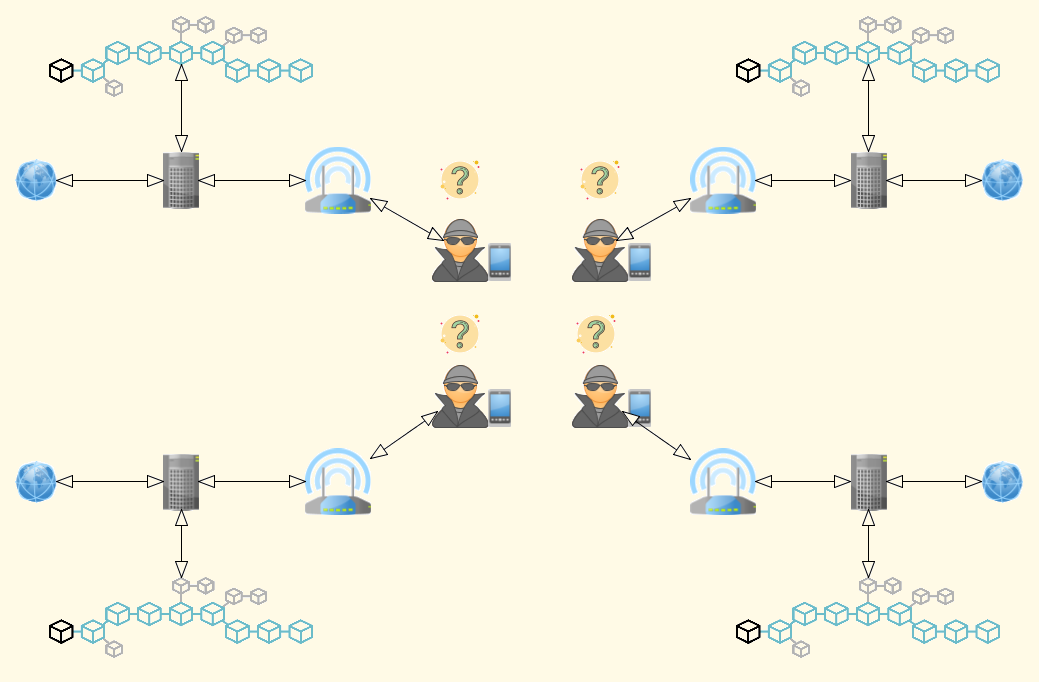
\includegraphics[keepaspectratio, width=0.8\textwidth]{images/bc5g/bc5g-y.eps}
  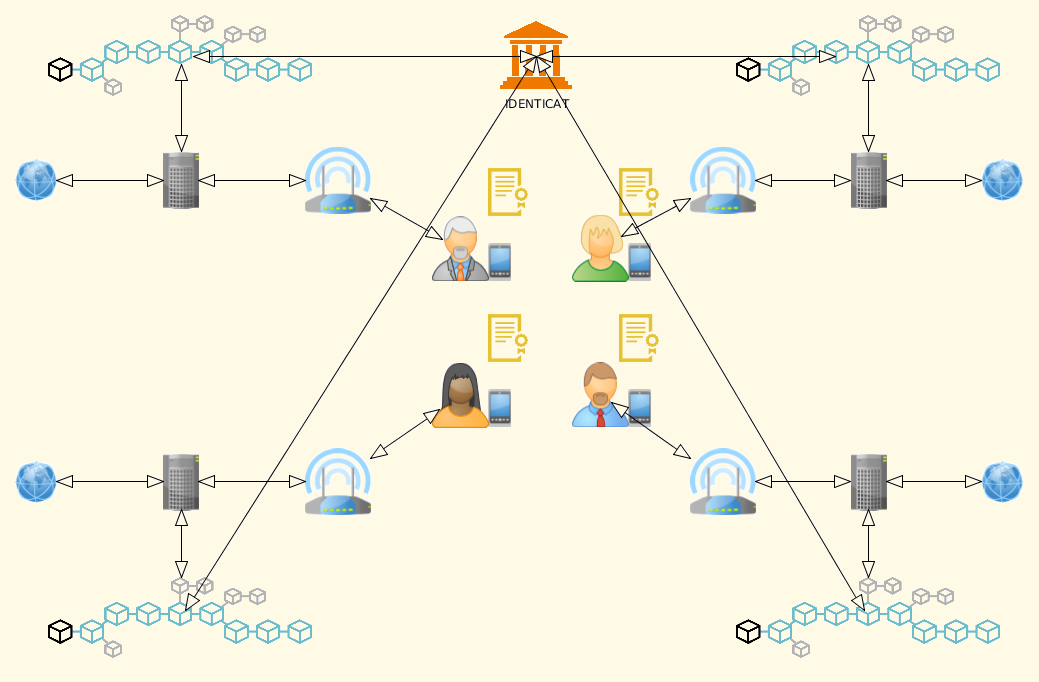
\includegraphics[keepaspectratio, width=0.8\textwidth]{images/bc5g/bc5g2-y.eps}
%  \caption{Figura 2. Raspberry Pi 3 Modelo B. Fuente: [Raspberry 18]}
%\end{figure}
\\
Figure 3. Anonymicity, identity, KyC and GDPR.
\\
\end{center}
\begin{multicols}{2}

\end{multicols}
\begin{center}
%\begin{figure}[h]
  %  \centering
  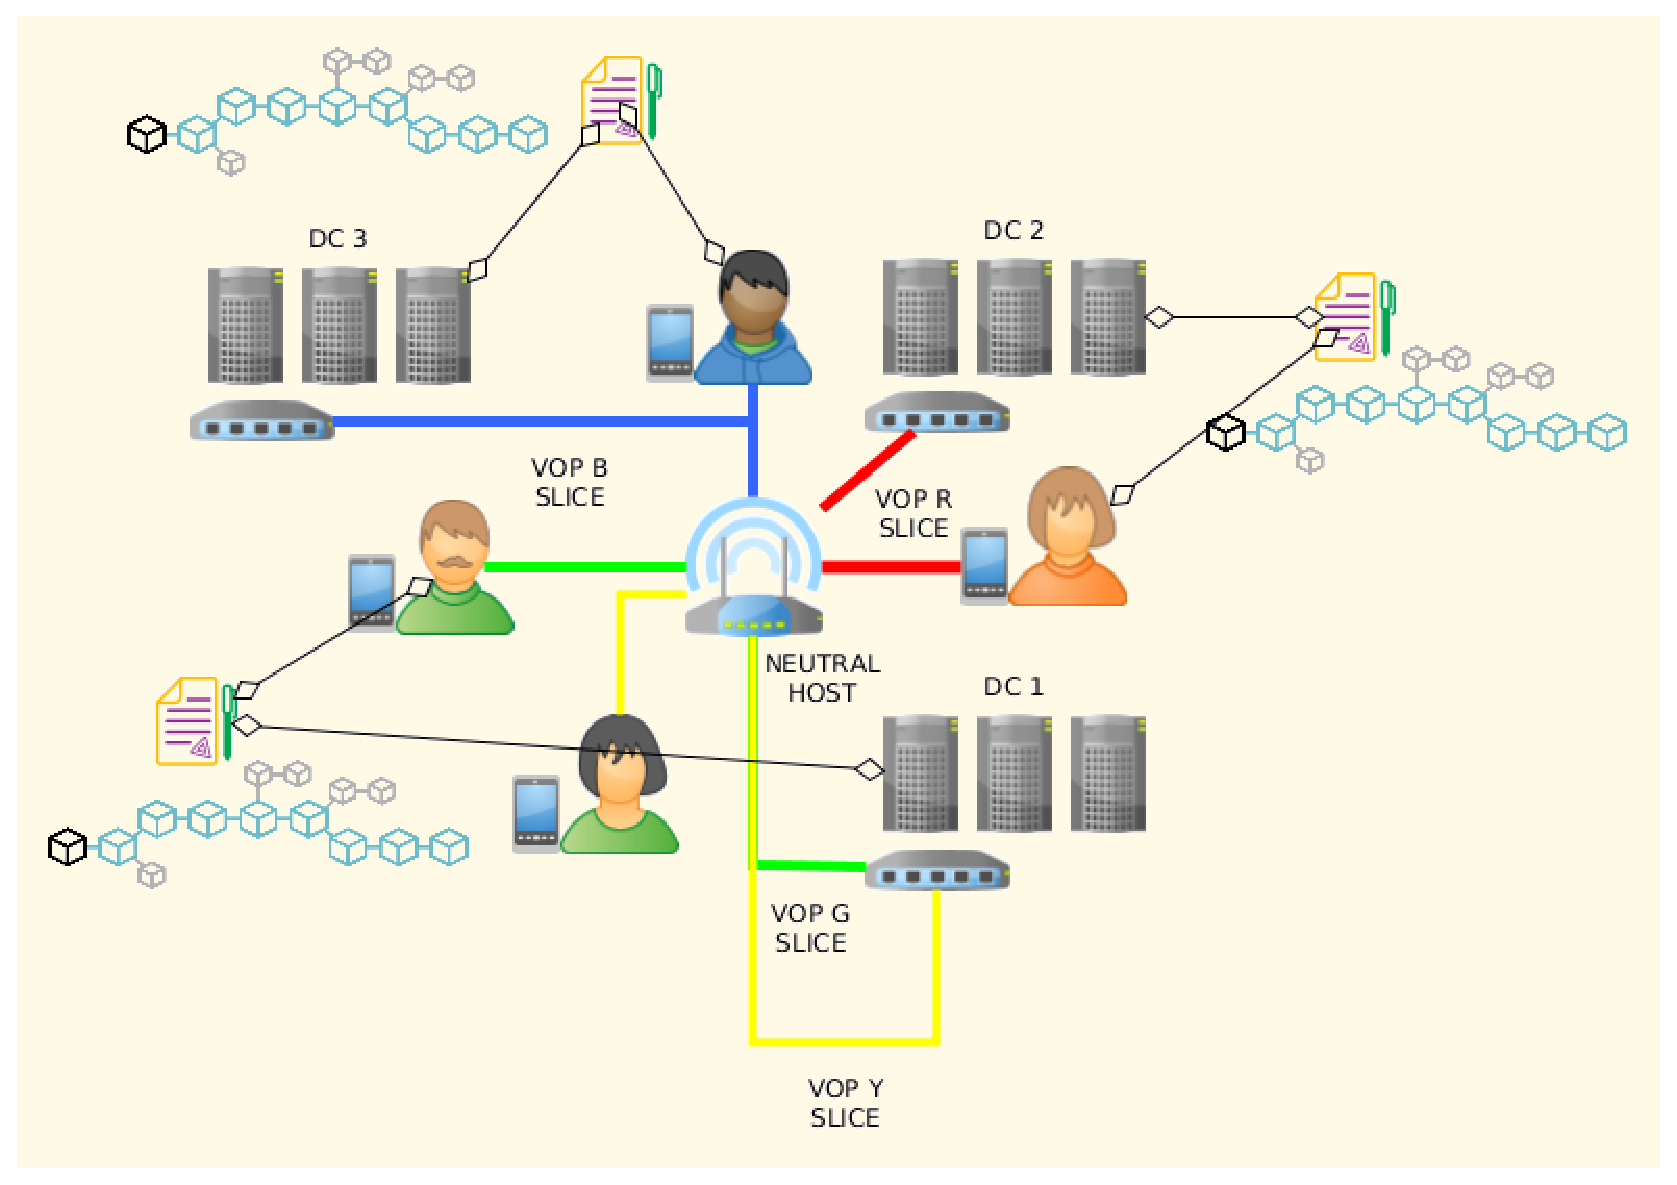
\includegraphics[keepaspectratio, width=0.8\textwidth]{images/bc5g/slices-y.eps}
%  \caption{Figura 2. Raspberry Pi 3 Modelo B. Fuente: [Raspberry 18]}
%\end{figure}
\\
Figure 4. Slicing model.
\\
\end{center}
\begin{multicols}{2}


\end{multicols}
\begin{center}
%\begin{figure}[h]
  %  \centering
  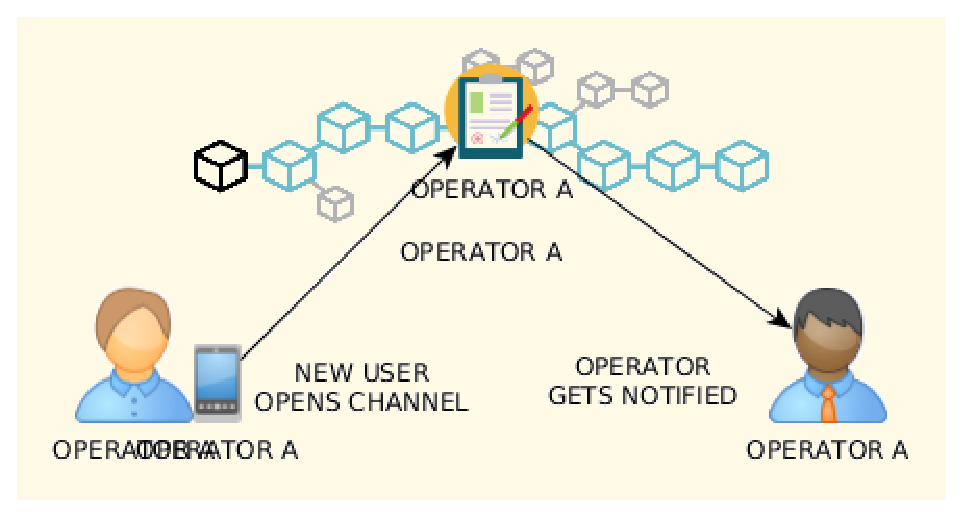
\includegraphics[keepaspectratio, width=0.6\textwidth]{images/bc5g/sc1-y.eps}
  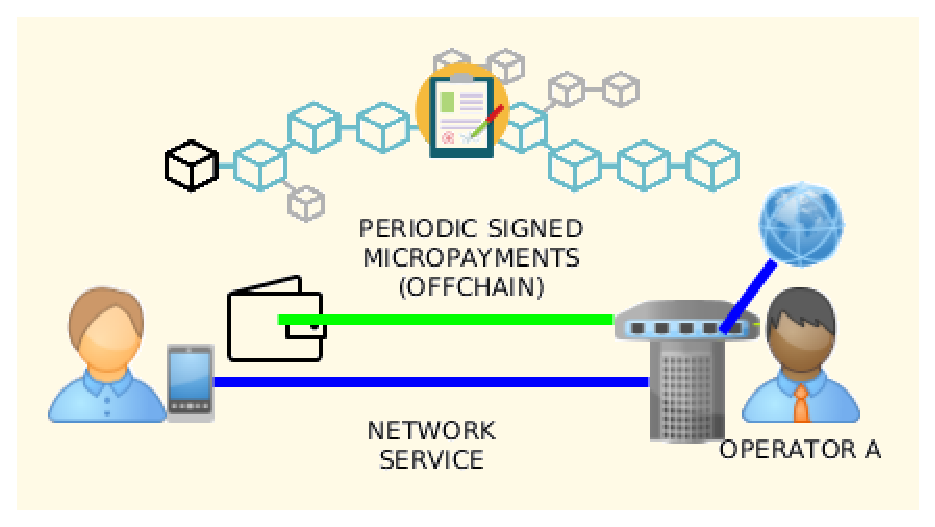
\includegraphics[keepaspectratio, width=0.6\textwidth]{images/bc5g/sc2-y.eps}
  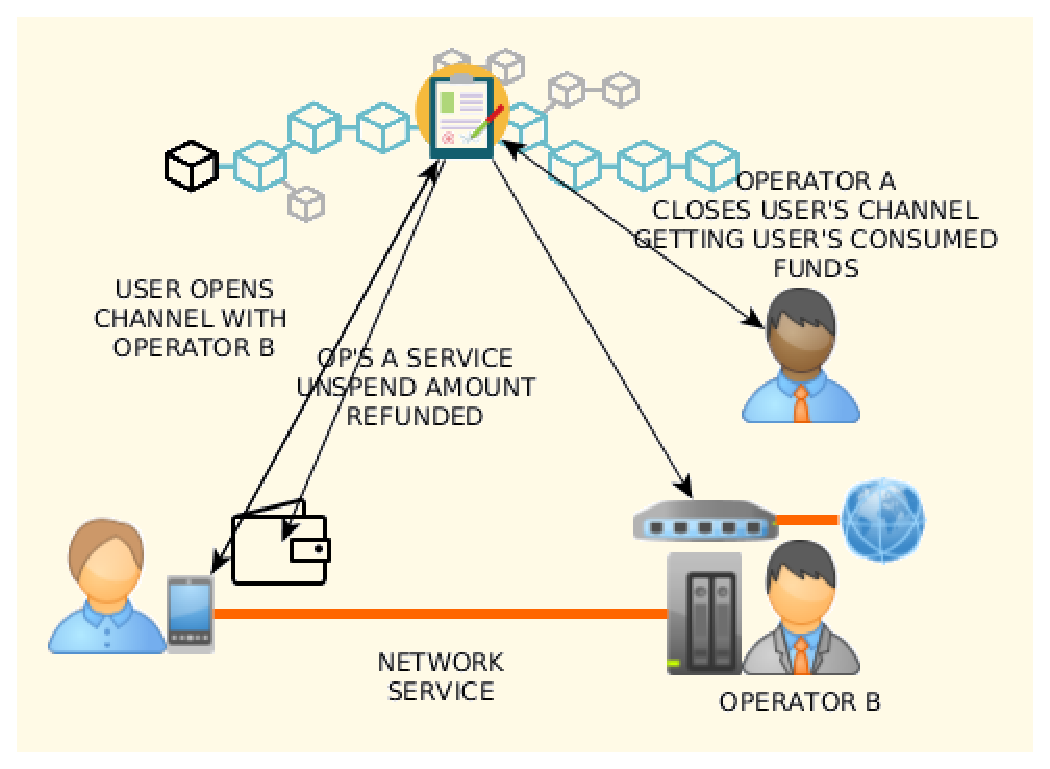
\includegraphics[keepaspectratio, width=0.6\textwidth]{images/bc5g/sc3-y.eps}
%  \caption{Figura 2. Raspberry Pi 3 Modelo B. Fuente: [Raspberry 18]}
%\end{figure}
\\
Figure 5. State channels support instant portability
between different operators with minimal fee.
\\
\end{center}
\begin{multicols}{2}


\end{multicols}
\begin{center}
%\begin{figure}[h]
  %  \centering
  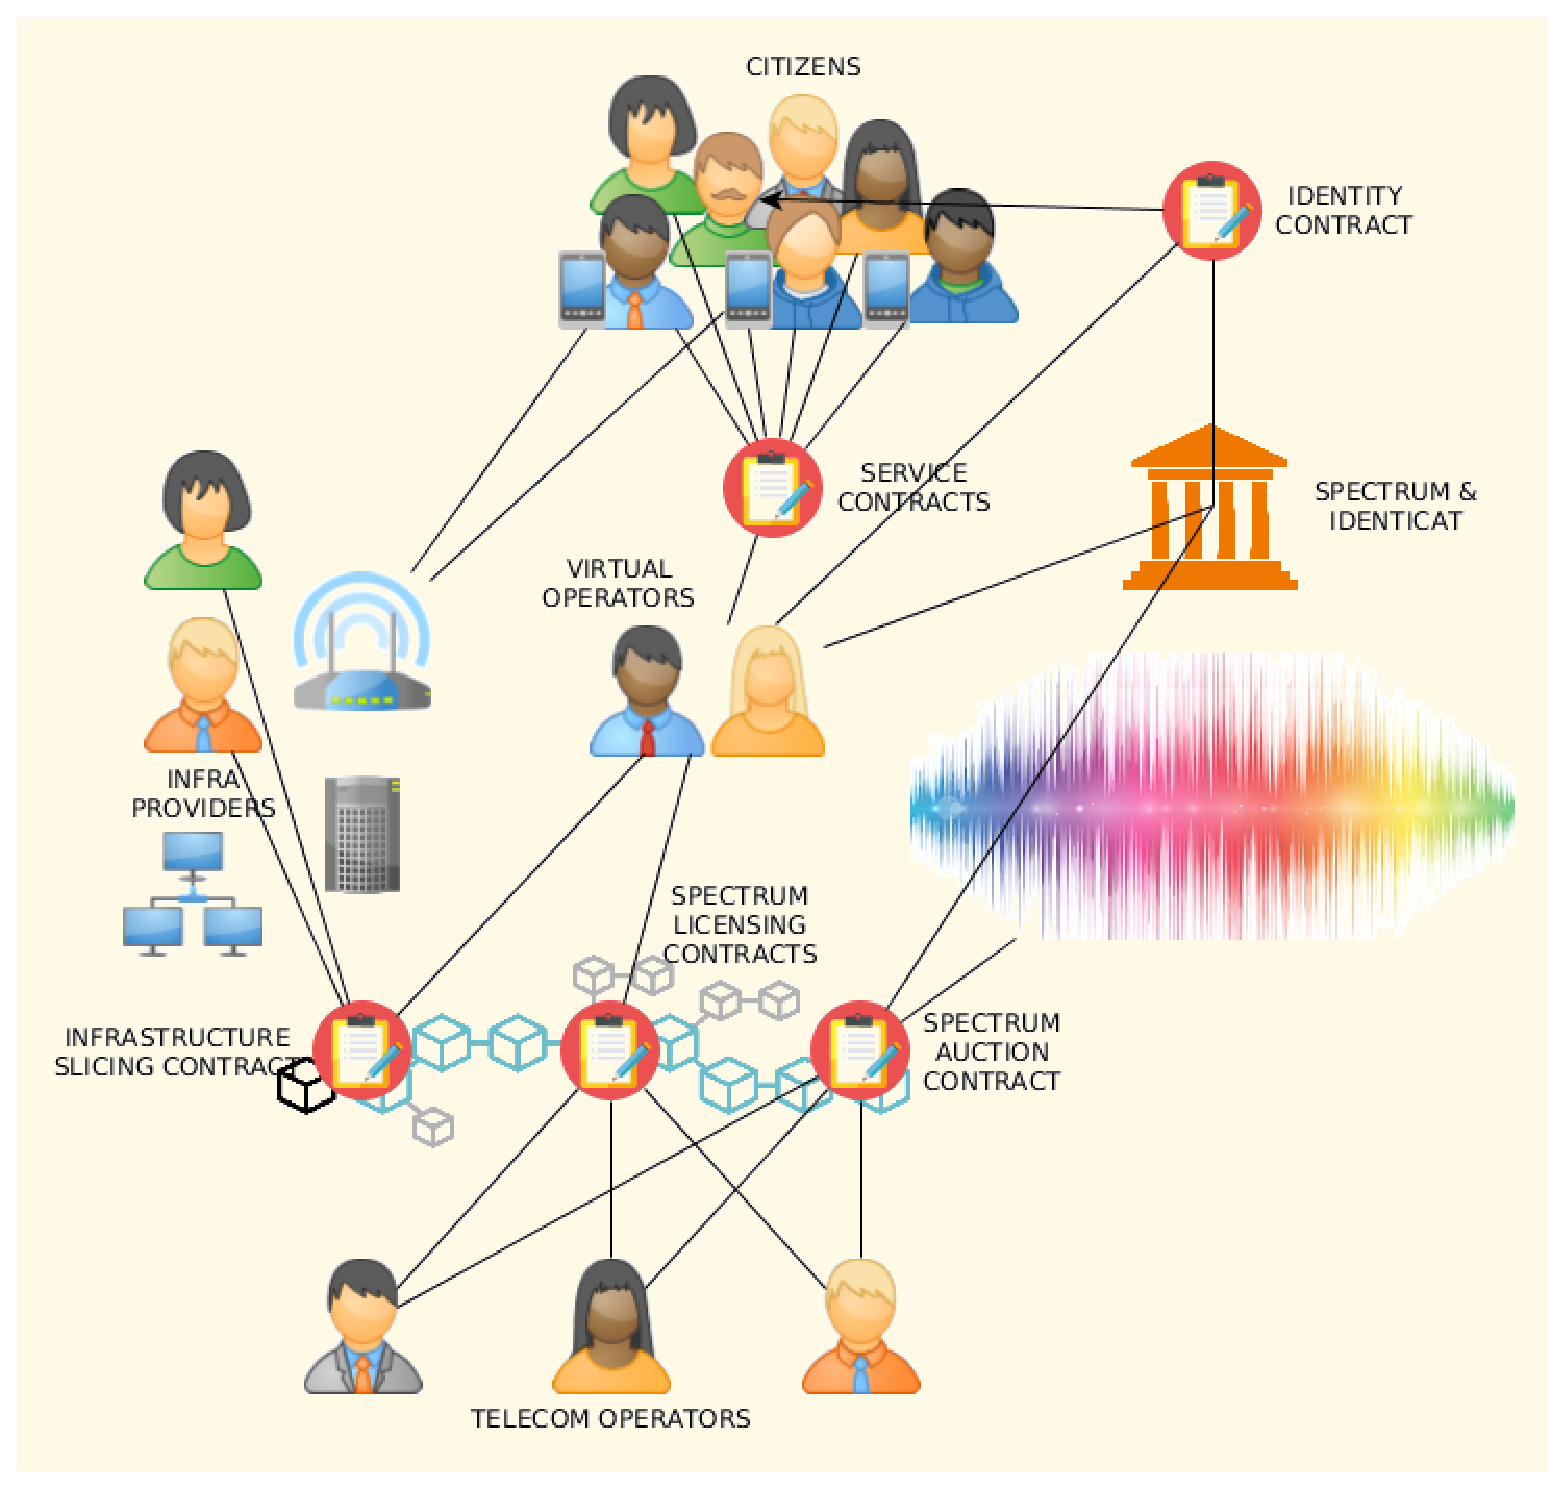
\includegraphics[keepaspectratio, width=0.8\textwidth]{images/bc5g/beyond-y.eps}
%  \caption{Figura 2. Raspberry Pi 3 Modelo B. Fuente: [Raspberry 18]}
%\end{figure}
\\
Figure 6. Full tokenization of wireless services from
the spectrum licensing to the citizen.
\\
\end{center}
\begin{multicols}{2}

%% Un resumen de sus especificaciones se da a continuación (véase tabla 1):
%% \begin{center}
%% %\begin{tabular} to 0.5\textwidth { | X[l] | X[r] | }
%% \begin{tabular}{ | m{0.125\textwidth} | m{0.3125\textwidth} | }
%%  \hline
%%  Especificaciones & Raspberry Pi 3 Modelo B \\
%%  \hline
%%  Procesador & Broadcom BCM2837, Cortex-A53 (ARMv8) 64-bit SoC @ 1,2 GHz \\
%% \hline
%%  RAM & 1 GB \\
%% \hline
%%  Conectividad & Wi-Fi 802.11 b/g/n (2,4 GHz) Bluetooth 4.1 Puerto Ethernet de hasta 100 Mbps \\
%% \hline
%%  Puertos & HDMI completo, 4 USB 2.0, MicroSD, CSI camera, DSI display \\
%% \hline
%%  Memoria & MicroSD \\
%% \hline
%% \end{tabular}
%% \newline
%% \end{center}
%% Tabla 1. Especificaciones de Raspberry Pi 3 Modelo B
%% %\newline
%% Aunque no se indica expresamente si es hardware libre (\textit{open hardware}) o con derechos de marca, en su página Web oficial explican que disponen de contratos de distribución y venta con dos empresas. Pero al mismo tiempo, cualquiera puede convertirse en revendedor o redistribuidor de las tarjetas Raspberry Pi [RaspberryPiBuy 19].

\vspace{0.35cm}

\subsubsection{Smart contract}
\subsubsection{Front-end} \label{ch:front-end}
\subsubsection{Back-end} \label{ch:back-end}

\subsection{Implementation} \label{ch:implementation}


\section{Quality considerations}\label{sec:proofs}
Para validar la PoC, se ha definido una batería de tests. Por ejemplo, dado que los smart contract normalmente manejan dinero, es esencial asegurarse de que su número de fallos y vulnerabilidades sea bajo [Hegedus 18]. Para ayudar a los desarrolladores y hacer más madura la tecnología, necesitamos herramientas de análisis [ConsenSys 19].
\subsection{Automated tests} \label{ch:tests}
(Por completar)

\section{Deployment}\label{sec:deploy}
Docker es una herramienta que permite desplegar aplicaciones dentro de contenedores de software. Esto puede ser útil para la Raspberry Pi porque permite a los usuarios ejecutar aplicaciones con muy poca sobrecarga, siempre y cuando la aplicación esté empaquetada dentro de una imagen Docker. Simplemente instalamos Docker y ejecutamos el contenedor sobre Raspbian/ARM. Éste despliega el proyecto realizado.

La secuencia de comandos a ejecutar es:
\\
\begin{flushleft}
\$ sudo apt-get install git
\\
\$ git clone https://github.com/ethereum-internet-access/docker.git
\\
\$ cd docker
\\
\$ sh ./install-project-inside-docker-container.sh
\end{flushleft}
\section{Viabilidad de negocio}\label{sec:business}
(Por completar)
\subsection{Legislación} \label{ch:legislation}
(Por completar)
\section{Conclusiones}\label{sec:conclusions}
El mundo en el que vivimos es interconectado.
En él Internet juega un papel fundamental.
Se ha contribuido a la construcción de
una PoC. Ésta se ha basado en la medida de
lo posible en hardware libre
(Raspberry Pi) ya que goza de buena popularidad
para el desarrollo de prototipos.
Como debilidad del pago con ETH, se puede
achacar la volatilidad de su precio (véase figura 3).
Esto conlleva variaciones en
las comisiones (\textit{fees}) de una transacción Ethereum.
\begin{center}
%\begin{figure}[h]
%  \centering
  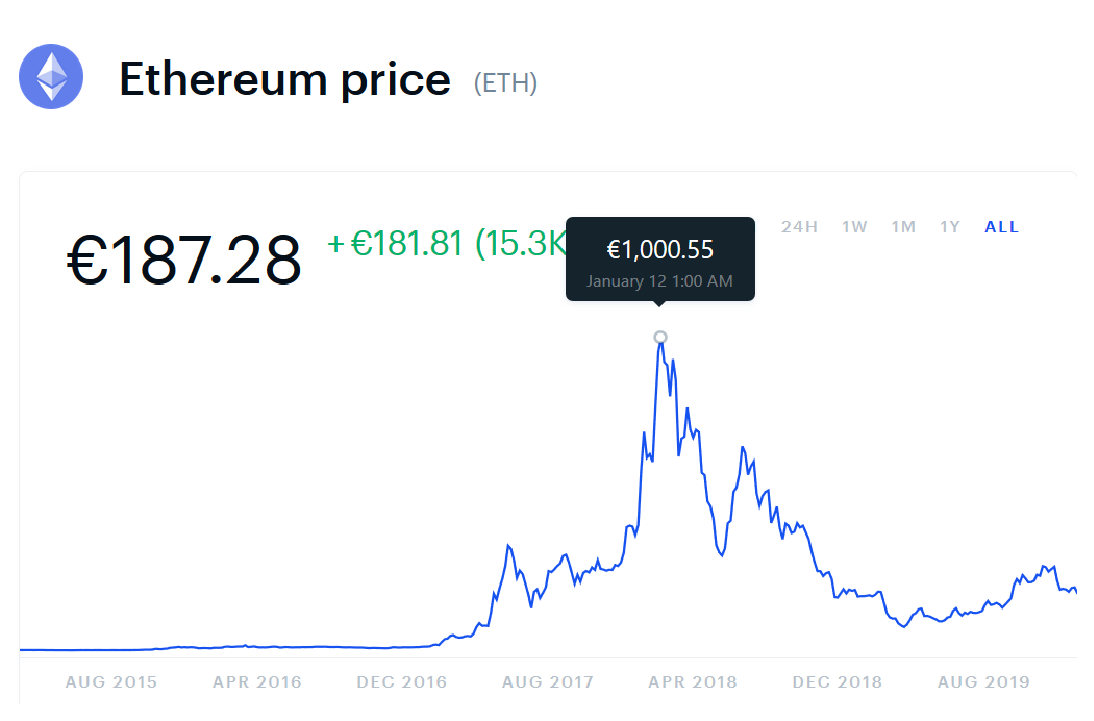
\includegraphics[keepaspectratio, width=0.481125\textwidth]{images/ethcurrentprice-sourcecoinbase.eps}
%  \caption{Figura 3. Variación cotización ETH (11/08/2019)}
%\end{figure}
\\
Figura 3. Variación cotización ETH (11/08/2019). Fuente: [Coinbase 19]
\\
\end{center}
(Por completar)
\section{Líneas futuras}\label{sec:future}
Como líneas futuras y complemento a este trabajo, con más tiempo, se plantea:
\subsection{Añadir forma de pago DAI} \label{ch:dai}
DAI es una criptomoneda estable (\textit{stablecoin}) que funciona con ETH y que intenta mantener un valor de 1\$. A diferencia de los billetes de banco centralizados, DAI no está respaldado por dólares estadounidenses en una cuenta bancaria. En cambio, está respaldado por garantías en la plataforma Maker [MakerDAO 19].
\subsection{Usar Raspberry Pi 4 Modelo B} \label{ch:rpi4modelb}
Anunciado en Junio de 2019 y a la venta. Es un hardware que ofrece mejores prestaciones. Por ejemplo, el procesador es un Broadcom BCM2711. Un ARM Cortex-A72 de cuatro núcleos y a 1,5 GHz. Hasta tres veces más eficiente (\textit{benchmark}) que el modelo anterior (Raspberry Pi 3 Modelo B+). También da la posibilidad de elegir entre 1, 2 y 4 GB de RAM.
\subsection{Usar Docker Swarm} \label{ch:dockerswarm}
Se podría presentar una aplicación descentralizada basada en microservicios. Por ejemplo en microservicios, un contenedor Docker (como en la sección 4) podría verse como un servicio. Entre las ventajas que aporta microservicios estarían:
\begin{itemize}
 \item Pequeños
 \item Independientes
 \item Despliegue sencillo
 \item Reutilizables
 \item Externalización
 \item Escalabilidad
 \newline
\end{itemize}
Para ello, Docker ofrece un orquestador (de código abierto) llamado Docker Swarm (véase figura 4). Un nodo \textit{worker} sería nuestra Raspberry Pi y un nodo \textit{manager} sería un centro de control.
\begin{center}
%\begin{figure}[h]
%  \centering
  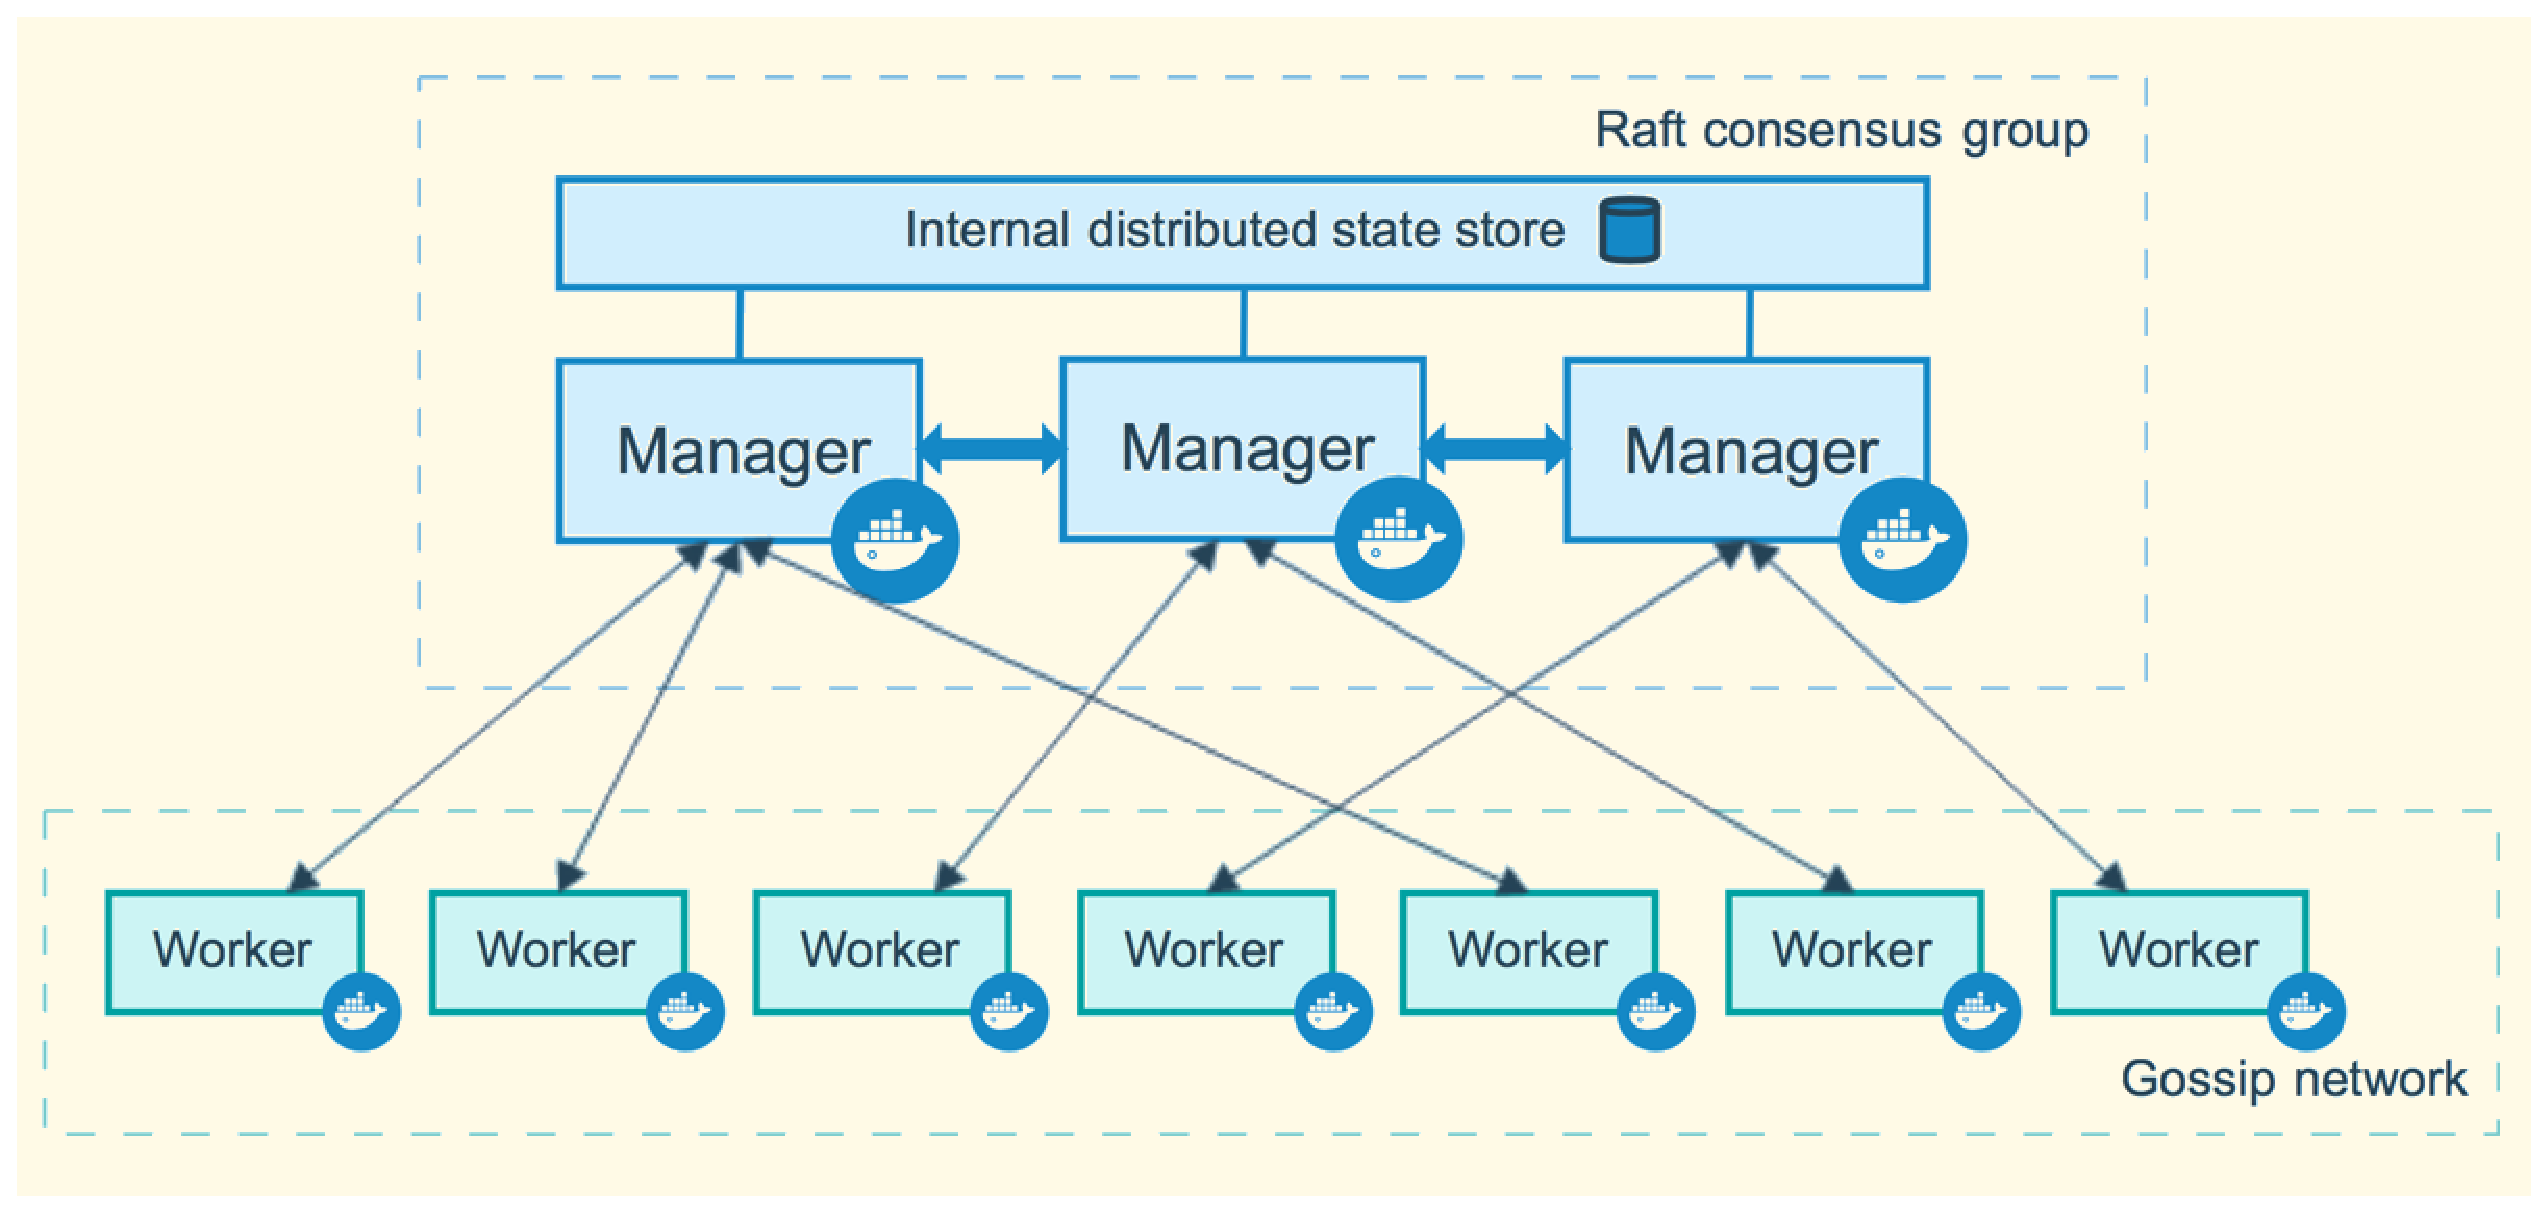
\includegraphics[keepaspectratio, width=0.481125\textwidth]{images/swarm-diagram-sourcedocker.eps}
%  \caption{Figura 3. Variación cotización ETH (11/08/2019)}
%\end{figure}
\\
Figura 4. Diagrama Docker Swarm. Fuente: [Docker 19]
\\
\end{center}
\section{Repositorio}\label{sec:repository}
El código fuente generado en el proyecto está publicado en un repositorio público de GitHub bajo licencia MIT.
\newline\newline
\url{https://github.com/ethereum-internet-access}
\newline
\begin{thebibliography}{9}
\bibitem{spectrumnh}
  \href{https://uk5g.org/media/uploads/resource_files/Spectrum\_NH\_discussion\_paper\_20Feb19.pdf}{5G Spectrum and Neutral Hosting}, Discussion paper, February 2019,
  DCMS Phase 1 5G Testbeds \& Trials Programme
\bibitem{5g} \href{https://en.wikipedia.org/wiki/5G}{https://en.wikipedia.org/wiki/5G}
\bibitem{sdns} Ian F. Akyildiz and Shih-Chun Lin and Pu Wang,
  \textit{Wireless software-defined networks (W-SDNs) and network function virtualization (NFV) for 5G cellular systems:
    An overview and qualitative evaluation}, Computer Networks, 93, 2015
\bibitem{nfv} Jose Ordonez-Lucena et al.
  \textit{Network Slicing for 5G with SDN/NFV: Concepts, Architectures, and Challenges},
   IEEE Communications Magazine ( Volume: 55 , Issue: 5 , May 2017 )
\bibitem{fon} \href{https://es.wikipedia.org/wiki/La_Fonera}{https://es.wikipedia.org/wiki/La\_Fonera}
\bibitem{hotspotme} \href{https://devpost.com/software/hotspot-me}{https://devpost.com/software/hotspot-me}
\bibitem{hostapd} \href{https://w1.fi/hostapd/}{https://w1.fi/hostapd/}
\bibitem{iptables} \href{https://linux.die.net/man/8/iptables}{https://linux.die.net/man/8/iptables}
\bibitem{dnsmasq} \href{https://en.wikipedia.org/wiki/Dnsmasq}{https://en.wikipedia.org/wiki/Dnsmasq}


\bibitem{Coinbase19} Coinbase. Intercambio de moneda digital \href{https://www.coinbase.com/price/ethereum}{https://www.coinbase.com/price/ethereum}
\bibitem{ConsenSys19} Ethereum Smart Contract Best Practices. Security tools. ConsenSys. 12 Agosto 2019.
\bibitem{Docker19} Docker Documentation. How nodes work. 6 Septiembre 2019.  \href{https://docs.docker.com/engine/swarm/how-swarm-mode-works/nodes/}{https://docs.docker.com/engine/swarm/how-swarm-mode-works/nodes/}
\bibitem{ETHBerlinZwei19} Hackathon ETH Berlín Zwei. Twitter. 6 Septiembre 2019. \href{https://twitter.com/ETHBerlin}{https://twitter.com/ETHBerlin}
\bibitem{Hegedus18} P. Hegedus. "Towards Analyzing the Complexity Landscape of Solidity Based Ethereum Smart Contracts". 2018 IEEE/ACM 1st International Workshop on Emerging Trends in Software Engineering for Blockchain (WETSEB). 27 Mayo-3 Junio 2018. \href{https://ieeexplore.ieee.org/document/8445056}{https://ieeexplore.ieee.org/document/8445056}
\bibitem{MakerDAO19} MakerDAO. Stability for the blockchain.  \href{https://makerdao.com/en/dai}{https://makerdao.com/en/dai}
\bibitem{Munoz18} J. L. Muñoz. "Docker Containers". Apuntes de las clases magistrales. Máster en Tecnologías Blockchain. 1, Edición. UPC School. 29 Noviembre 2018.
\bibitem{Nakamoto08} S. Nakamoto. "Bitcoin: A Peer-to-Peer Electronic Cash System". 31 Octubre 2008.  \href{https://bitcoin.org/bitcoin.pdf}{https://bitcoin.org/bitcoin.pdf}
\bibitem{RaspberryPi19} Raspberry Pi 3 Modelo B - Placa Base (1,2 GHz Quad-Core Arm Cortex-A53, 1 GB RAM, USB 2.0). Amazon. 11 Agosto 2019.
\bibitem{RaspberryPiBuy19} Raspberry Pi FAQs. BUYING AND SHIPPING. Where can I buy a Raspberry Pi?. Página Web oficial. 11 Agosto 2019.  \href{https://www.raspberrypi.org/help/faqs/#buyingWhere}{https://www.raspberrypi.org/help/faqs/\#buyingWhere}
\bibitem{Stallings04} W. Stallings. "Comunicaciones y redes de computadores". 1 Septiembre 2004. Páginas 904. Pearson Prentice Hall. ISBN-13: 978-8420541105.
\end{thebibliography}
\clearpage


\end{multicols}


\end{document}
